\documentclass{beamer}

\usetheme{metropolis} % Você pode trocar o tema por: Warsaw, AnnArbor, CambridgeUS, etc.

\title{Controle \textit{Go-to-Goal} para Robôs com tração diferencial usando critério de estabilidade de Lyapunov}
\author{Matheus L. T. Farias}
\institute{Automação Inteligente}
\date{24 de Julho de 2025}

\begin{document}

%======================================================================
\frame{\titlepage}
%======================================================================
% Seção: Introdução
\section{Introdução}

\begin{frame}{Motivação}
  \begin{itemize}
    \item Robôs móveis autônomos enfrentam desafios de controle devido a restrições não-holonômicas.
    \item O controle preciso é essencial em aplicações como:
    \begin{itemize}
        \item Veículos autônomos
        \item Robôs de vigilância
        \item Robôs assistivos
    \end{itemize}
    \item Métodos com garantias formais de estabilidade são desejáveis.
  \end{itemize}
\end{frame}
%======================================================================
\begin{frame}{Objetivos do Trabalho}
  \begin{itemize}
    \item Implementar leis de controle para o modelo cinemático Uniciclo para o problema do tipo \textit{Go-to-Goal}\ seguindo duas abordagens:
    \begin{itemize}
        \item Aicardi et al. (1995)
        \item Benbouabdallah et al. (2013)
    \end{itemize}
    \item Utilizar o critério de estabilidade de Lyapunov para garantir convergência assintótica.
    \item Verificar a eficácia das abordagens.
    \item Comparar o desempenho das abordagens propostas.
    \item Utilizar o ambiente CoppeliaSim para validação experimental.
  \end{itemize}
\end{frame}
%======================================================================

% Seção: Fundamentação Teórica
\section{Fundamentação Teórica}

\begin{frame}{Estabilidade de Lyapunov}
  \begin{itemize}
    \item A teoria de Lyapunov permite verificar a estabilidade de sistemas dinâmicos sem resolver suas equações diferenciais.
    \item Baseia-se na definição de uma função escalar $V(x)$, chamada de \textbf{função de Lyapunov}.
    \item O sistema é estável se:
    \begin{itemize}
      \item $V(x) > 0$ para todo $x \neq 0$ e $V(0) = 0$ (positividade definida)
      \item $\dot{V}(x) \leq 0$ para todo $x$ (derivada negativa semi-definida)
    \end{itemize}
  \end{itemize}
\end{frame}
%======================================================================
\begin{frame}{Estabilidade Assintótica}
  \begin{itemize}
    \item Se $\dot{V}(x) < 0$ para todo $x \neq 0$, a estabilidade é \textbf{assintótica}.
    \item Isso significa que as trajetórias convergem para o ponto de equilíbrio ao longo do tempo.
    \item Utilizado especialmente para sistemas não lineares.
  \end{itemize}

  \vspace{0.5cm}
  \textbf{Exemplo de sistema dinâmico:}
  \[
  \dot{x} = f(x), \quad x \in \mathbb{R}^n,\quad f(0) = 0
  \]
\end{frame}
%======================================================================
\begin{frame}{Função de Lyapunov Quadrática}
  \begin{itemize}
    \item Uma escolha comum para sistemas lineares:
    \[
    V(x) = x^\top P x
    \]
    \item Onde $P \in \mathbb{R}^{n \times n}$ é simétrica e definida positiva ($P = P^\top > 0$).
    \item A derivada temporal de $V$ pode ser obtida como:
    \[
    \dot{V}(x) = \dot{x}^\top P x + x^\top P \dot{x}
    \]
    \item Essa estrutura é base para projetar leis de controle estáveis.
  \end{itemize}
\end{frame}
%======================================================================

% Seção: Modelo Cinemático do Robô
\section{Modelo Cinemático do Robô}

\begin{frame}{Equações do Modelo Cinemático}
  \begin{itemize}
    \item O modelo de cinemático Uniciclo é dado pela equação abaixo, considerando um vetor de estados $q$:
    \[
    \begin{cases}
        \dot{x} = v \cos \theta \\
        \dot{y} = v \sin \theta \\
        \dot{\theta} = \omega
    \end{cases},\quad \quad
    q = \begin{bmatrix} x \\ y \\ \theta \end{bmatrix}
    \]
    \item Onde:
    \begin{itemize}
      \item $(x, y)$: posição do robô no plano
      \item $\theta$: orientação do robô em relação ao eixo $x$ global
    \end{itemize}
    \item Entradas de controle:
    \begin{itemize}
      \item $v$: velocidade linear
      \item $\omega$: velocidade angular
    \end{itemize}
  \end{itemize}
\end{frame}
%======================================================================
\begin{frame}{Aplicação da Teoria de Lyapunov}
  \begin{itemize}
    \item A estrutura do modelo é compatível com sistemas da forma $\dot{x} = f(x)$.
    \item Isso permite aplicar a teoria de Lyapunov para projetar leis de controle para $v$ e $\omega$.
    \item O objetivo é garantir estabilidade assintótica em relação a uma pose alvo desejada.
  \end{itemize}
\end{frame}
%======================================================================
% Seção: Problema do Estacionamento
\section{Problema do Estacionamento}

\begin{frame}{Definição do Problema}
  \begin{itemize}
    \item O problema do estacionamento consiste em levar o robô de uma pose inicial qualquer até uma pose desejada $(x_T, y_T)$.
    \item Requer o controle tanto da posição quanto da orientação final do robô.
    \item Importante: deve-se garantir estabilidade do sistema durante todo o movimento.
  \end{itemize}
\end{frame}

\begin{frame}{Abordagens Consideradas}
  Neste trabalho, o problema do estacionamento é tratado com base em duas abordagens da literatura:
  \begin{itemize}
    \item \textbf{Aicardi et al. (1995)}:
    \begin{itemize}
      \item Foca na estabilização assintótica para alvos fixos.
    \end{itemize}
    \item \textbf{Benbouabdallah et al. (2013)}:
    \begin{itemize}
      \item Originalmente proposta para rastreamento de alvos móveis.
      \item Aplicada aqui ao caso particular de alvos fixos.
    \end{itemize}
  \end{itemize}
\end{frame}

\begin{frame}{Objetivo da Solução de Controle}
  \begin{itemize}
    \item Projetar leis de controle para $v$ (linear) e $\omega$ (angular) que:
    \begin{itemize}
      \item Garantam a convergência do robô à posição e orientação desejadas.
      \item Satisfaçam os critérios de estabilidade de Lyapunov.
    \end{itemize}
  \end{itemize}
\end{frame}
%======================================================================
% Seção: Abordagem de Aicardi et al.
\section{Abordagem de Aicardi et al.}

\begin{frame}{Visão Geral da Abordagem}
\begin{figure}[h!]
    \centering
    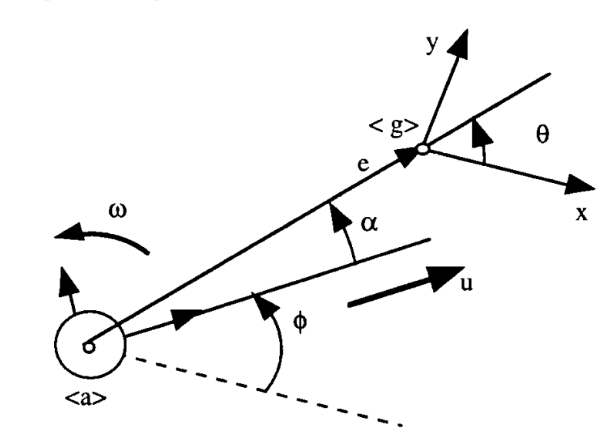
\includegraphics[width=0.6\textwidth]{Figuras/Sistema_Robo_Alvo.png}
    \caption{Sistema Robô-Alvo}
    \label{fig:Sistema_Robo_Alvo}
\end{figure}
  \begin{itemize}
    \item Baseada em uma reformulação do sistema em coordenadas relativas ao alvo.
  \end{itemize}
\end{frame}

\begin{frame}{Redefinição de Variáveis}
  \begin{itemize}
    \item Variáveis relativas:
    \begin{itemize}
      \item $e$: distância entre o robô e o alvo
      \item $\theta$: orientação desejada
      \item $\phi$: orientação atual do robô
      \item $\alpha = \theta - \phi$: erro angular
    \end{itemize}
    \item Vetor de estado:
    \[
    x = \begin{bmatrix} e \\ \alpha \\ \theta \end{bmatrix}
    \]
    \item O ponto de equilíbrio desejado é $x = [0, 0, \theta]^T$.
  \end{itemize}
\end{frame}

\begin{frame}{Função de Lyapunov Proposta}
  \[
  V = \frac{1}{2} \lambda e^2 + \frac{1}{2}(\alpha^2 + h \theta^2), \quad \lambda, h > 0
  \]

  \begin{itemize}
    \item Baseado numa forma quadrática com:
    \[
    x = \begin{bmatrix} e \\ \alpha \\ \theta \end{bmatrix}, \quad
    P =
    \begin{bmatrix}
        \dfrac{1}{2}\lambda & 0 & 0\\
        0 & \dfrac{1}{2} & 0\\
        0 & 0 & \dfrac{1}{2}h
    \end{bmatrix}
    \]
  \end{itemize}
\end{frame}

\begin{frame}{Derivada de Lyapunov}
  \begin{equation*}
  \dot{V} = -\lambda e u \cos(\alpha) + \alpha \left[ -\omega + \frac{u}{e} \sin(\alpha) \cdot \frac{\alpha + h\theta}{\alpha} \right]
  \end{equation*}

  \begin{itemize}
    \item O objetivo é projetar $u$ e $\omega$ para que $\dot{V} < 0$ para todo $x \neq 0$.
  \end{itemize}
\end{frame}

\begin{frame}{Leis de Controle Propostas}
  \[
  \begin{cases}
  u = \gamma e \cos(\alpha), \quad \gamma > 0 \\
  \omega = k\alpha + \gamma \frac{\sin(\alpha) \cos(\alpha)}{\alpha} (\alpha + h\theta)
  \end{cases}
  \]

  \begin{itemize}
    \item Substituindo essas leis em $\dot{V}$, obtém-se:
    \[
    \dot{V} = -\lambda \gamma e^2 \cos^2(\alpha) - k\alpha^2 \leq 0
    \]
    \item Estabilidade assintótica garantida pela teoria de Lyapunov.
  \end{itemize}
\end{frame}
%======================================================================
% Seção: Abordagem de Benbouabdallah et al.
\section{Abordagem de Benbouabdallah et al.}

\begin{frame}{Visão Geral da Abordagem}

\begin{figure}[h!]
    \centering
    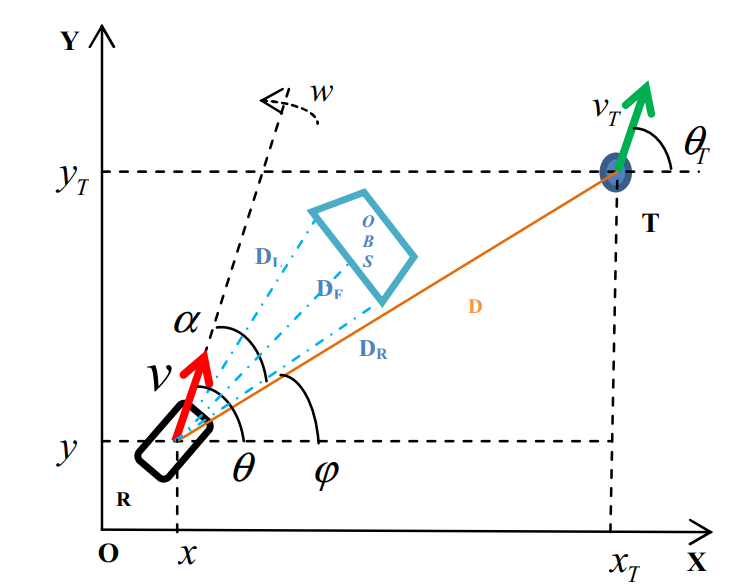
\includegraphics[width=0.55\textwidth]{Figuras/Sistema_Robo_Albo_2.png}
    \caption{Sistema Robô-Alvo}
    \label{fig:Sistema_Robo_Alvo_2}
\end{figure}

  \begin{itemize}
    \item Utiliza um modelo geométrico com variáveis relativas entre o robô e o alvo.
  \end{itemize}
\end{frame}

\begin{frame}{Variáveis Geométricas}
  \begin{itemize}
    \item Variáveis relativas:
    \begin{itemize}
      \item $D$: distância entre o robô e o alvo
      \item $\theta$: orientação atual do robô
      \item $\phi$: orientação desejada
      \item $\alpha = \theta - \phi$: erro angular
    \end{itemize}
     \item Erros definidos como:
    \[
    e_D = D_d - D, \quad
    e_\alpha = \alpha_d - \alpha
    \]
    \item Vetor de estado:
    \[
    x = \begin{bmatrix} e_D \\ e_\alpha\end{bmatrix}
    \]
    \item O ponto de equilíbrio desejado é $x = [0, 0]^T$.
  \end{itemize}
\end{frame}

\begin{frame}{Função de Lyapunov Proposta}
  \[
  V = \frac{1}{2} e_D^2 + \frac{1}{2} e_\alpha^2
  \]

    \begin{itemize}
        \item Baseado numa forma quadrática com:
        \[
        x = \begin{bmatrix} e_D \\ e_\alpha\end{bmatrix}, \quad
        P =
        \begin{bmatrix}
        \dfrac{1}{2} & 0 \\
        0 & \dfrac{1}{2}
        \end{bmatrix}
        \]
    \end{itemize}
\end{frame}

\begin{frame}{Derivada de Lyapunov}
  \[
  \dot{V} = e_D v\cos\alpha + \alpha\left(w - \dfrac{v}{D}\sin\alpha\right)
  \]

  Com: $\alpha_d$ = 0

  \begin{itemize}
    \item O objetivo é projetar $v$ e $w$ para que $\dot{V} < 0$ para todo $x \neq 0$.
  \end{itemize}
  
\end{frame}

\begin{frame}{Leis de Controle Propostas}
  \[
  \begin{cases}
  v = -K_v e_D \cos \alpha \\
  \omega = -K_\omega \alpha - \dfrac{v}{D} \sin \alpha
  \end{cases}, \quad K_v, K_\omega > 0
  \]

  Substituindo em $\dot{V}$:
  \[
  \dot{V} = -K_v e_D^2 \cos^2 \alpha - K_\omega \alpha^2 \leq 0
  \]

  \begin{itemize}
    \item Garante estabilidade assintótica.
  \end{itemize}
\end{frame}
%======================================================================
% Seção: Implementação e Simulação
\section{Implementação e Simulação}

\begin{frame}{Ambiente de Simulação}
  \begin{itemize}
    \item As leis de controle foram implementadas no simulador \textbf{CoppeliaSim}.
    \item Robô utilizado: \textbf{Pioneer 3-DX}, com tração diferencial.
    \item Informações de posição e orientação foram obtidas com sensores virtuais:
    \begin{itemize}
      \item \texttt{sim.getObjectPosition()}
      \item \texttt{sim.getObjectOrientation()}
    \end{itemize}
  \end{itemize}
\end{frame}

\begin{frame}{Conversão de Velocidades}
  \begin{itemize}
    \item O controle direto do robô no simulador é feito via velocidade angular das rodas ($\omega_R$, $\omega_L$).
    \item As leis de controle fornecem $v$ (linear) e $\omega$ (angular).
    \item Conversão para controle das rodas:
    \[
    \begin{cases}
    \omega_R = \dfrac{2v + \omega L}{2R} \\
    \omega_L = \dfrac{2v - \omega L}{2R}
    \end{cases}
    \]
    \item Onde:
    \begin{itemize}
      \item $L$: distância entre rodas (eixo)
      \item $R$: raio das rodas
    \end{itemize}
  \end{itemize}
\end{frame}

\begin{frame}{Cenários de Teste}
  \begin{itemize}
    \item Foram realizados testes em 4 cenas com posições iniciais distintas.
    \item A posição inicial do robô é fixa, mas o alvo muda:
    \begin{itemize}
      \item Cena 1: Alvo à frente
      \item Cena 2: Alvo ao lado
      \item Cena 3: Alvo na diagonal
      \item Cena 4: Alvo atrás do robô
    \end{itemize}
    \item Cada abordagem foi testada com os mesmos parâmetros em todas as cenas.
  \end{itemize}
\end{frame}

\begin{frame}{Parâmetros de Controle}
  \begin{itemize}
    \item \textbf{Aicardi et al.}
    \[
    \gamma = 0.1, \quad k = 1, \quad h = 1
    \]
    \item \textbf{Benbouabdallah et al.}
    \[
    K_v = 0.1, \quad K_\omega = 1
    \]
    \item Valores escolhidos arbitrariamente, respeitando a condição de estabilidade.
  \end{itemize}
\end{frame}

\begin{frame}{Cenas de Teste}
\begin{minipage}{0.48\linewidth}
    \centering
    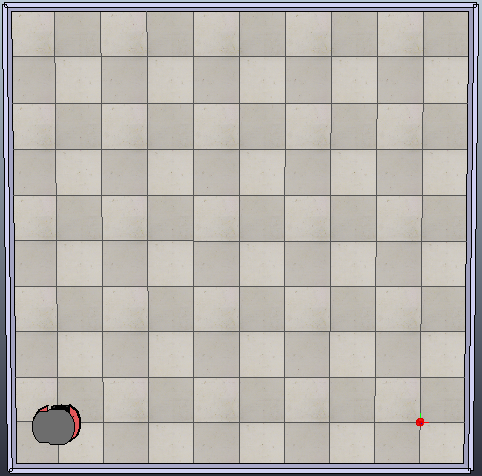
\includegraphics[width=\linewidth]{Figuras/Cena_teste_1.png}
   Cena de Teste 1
  \end{minipage}
  \hfill
  \begin{minipage}{0.48\linewidth}
    \centering
    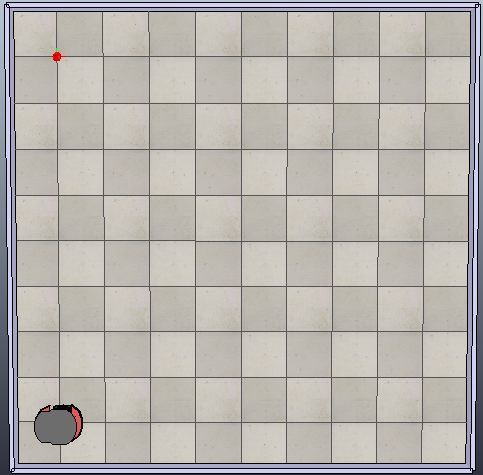
\includegraphics[width=\linewidth]{Figuras/Cena_teste_2.png}
    Cena de Teste 2
  \end{minipage}
\end{frame}

\begin{frame}{Cenas de Teste}
\begin{minipage}{0.48\linewidth}
    \centering
    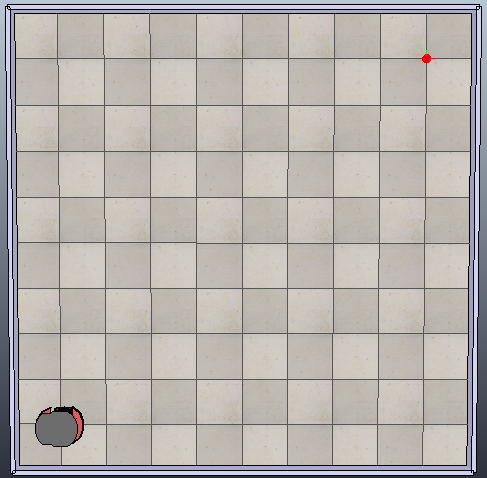
\includegraphics[width=\linewidth]{Figuras/Cena_teste_3.png}
   Cena de Teste 3
  \end{minipage}
  \hfill
  \begin{minipage}{0.48\linewidth}
    \centering
    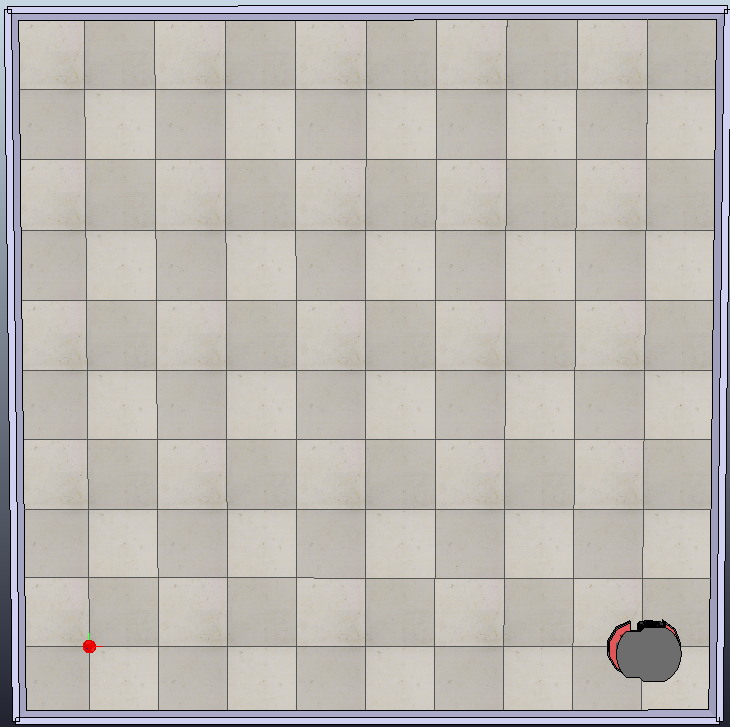
\includegraphics[width=\linewidth]{Figuras/Cena_teste_4.png}
    Cena de Teste 4
  \end{minipage}
\end{frame}


%======================================================================
% Seção: Resultados
\section{Resultados}

\begin{frame}{Trajetória do Robô}
  \begin{itemize}
    \item A trajetória do robô foi registrada em todas as cenas de teste.
    \item Cada abordagem gerou um padrão diferente de movimento.
    \item Os triângulos indicam a posição e orientação do robô, inseridos a cada 1,5 segundos para análise temporal.
  \end{itemize}
\end{frame}

\begin{frame}{Trajetória do Robô}
\begin{minipage}{0.48\linewidth}
    \centering
    \includegraphics[width=\linewidth]{Figuras/Tragetória_Cena_1.png}
  \end{minipage}
  \hfill
  \begin{minipage}{0.48\linewidth}
    \centering
    \includegraphics[width=\linewidth]{Figuras/Tragetória_Cena_2.png}
  \end{minipage}
\end{frame}

\begin{frame}{Trajetória do Robô}
\begin{minipage}{0.48\linewidth}
    \centering
    \includegraphics[width=\linewidth]{Figuras/Tragetória_Cena_3.png}
  \end{minipage}
  \hfill
  \begin{minipage}{0.48\linewidth}
    \centering
    \includegraphics[width=\linewidth]{Figuras/Tragetória_Cena_4.png}
  \end{minipage}
\end{frame}

\begin{frame}{Comandos de Controle}
  \begin{itemize}
    \item As figuras mostram a evolução desses sinais em cada cenário.
    \item Comandos analisados: $v(t)$ e $\omega(t)$
  \end{itemize}
\end{frame}

\begin{frame}{Comandos de Controle}
\begin{minipage}{0.48\linewidth}
    \centering
    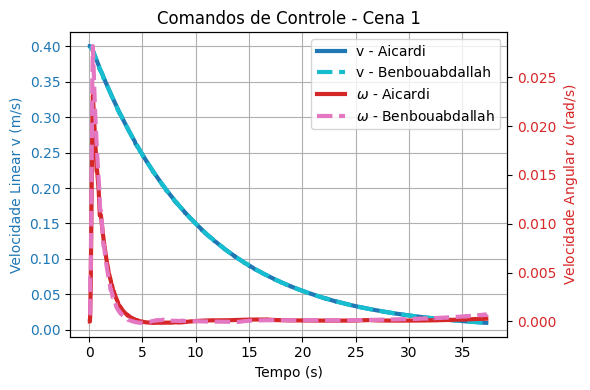
\includegraphics[width=\linewidth]{Figuras/Controle_Cena_1.png}
  \end{minipage}
  \hfill
  \begin{minipage}{0.48\linewidth}
    \centering
    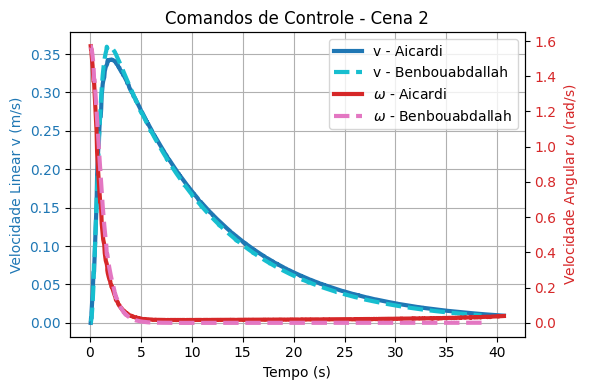
\includegraphics[width=\linewidth]{Figuras/Controle_Cena_2.png}
  \end{minipage}
\end{frame}

\begin{frame}{Comandos de Controle}
\begin{minipage}{0.48\linewidth}
    \centering
    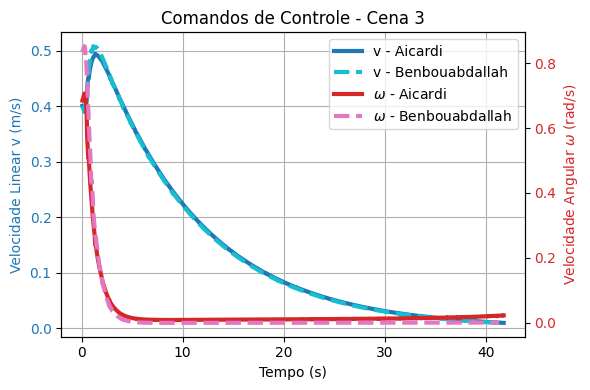
\includegraphics[width=\linewidth]{Figuras/Controle_Cena_3.png}
  \end{minipage}
  \hfill
  \begin{minipage}{0.48\linewidth}
    \centering
    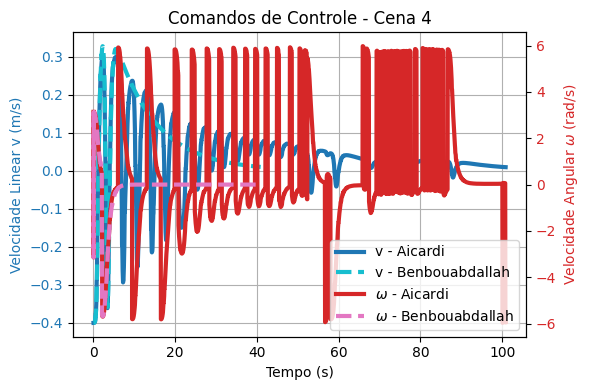
\includegraphics[width=\linewidth]{Figuras/Controle_Cena_4.png}
  \end{minipage}
\end{frame}

\begin{frame}{Erro de Posição}
  \begin{itemize}
    \item A distância entre o robô e o alvo foi monitorada durante a simulação.
  \end{itemize}
\end{frame}

\begin{frame}{Erro de Posição}
\begin{minipage}{0.48\linewidth}
    \centering
    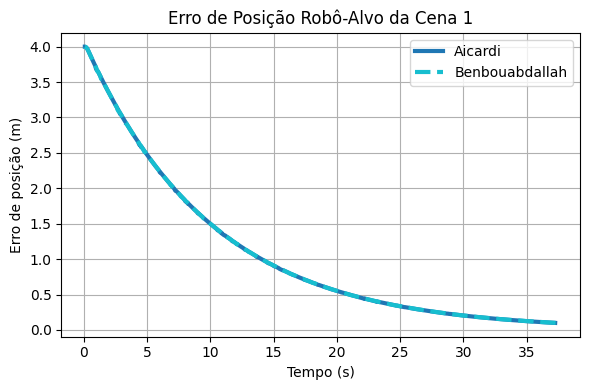
\includegraphics[width=\linewidth]{Figuras/ErroPosição_Cena_1.png}
  \end{minipage}
  \hfill
  \begin{minipage}{0.48\linewidth}
    \centering
    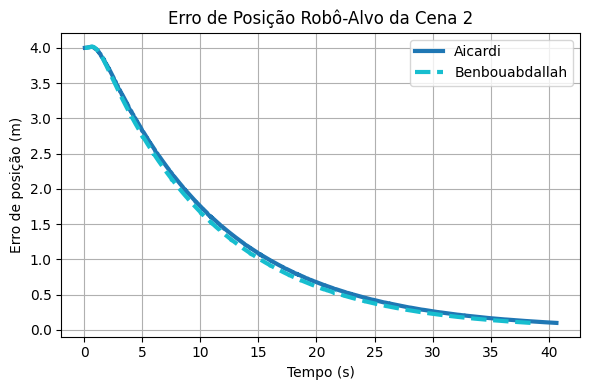
\includegraphics[width=\linewidth]{Figuras/ErroPosição_Cena_2.png}
  \end{minipage}
\end{frame}

\begin{frame}{Erro de Posição}
\begin{minipage}{0.48\linewidth}
    \centering
    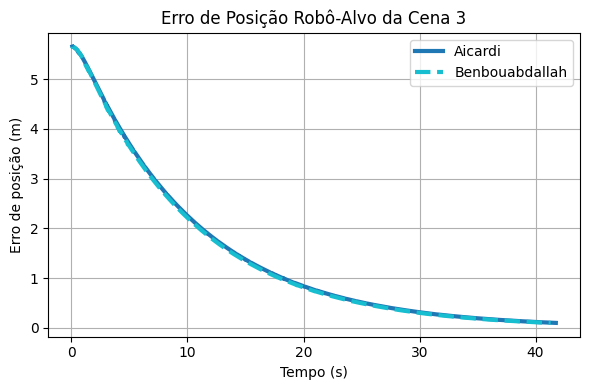
\includegraphics[width=\linewidth]{Figuras/ErroPosição_Cena_3.png}
  \end{minipage}
  \hfill
  \begin{minipage}{0.48\linewidth}
    \centering
    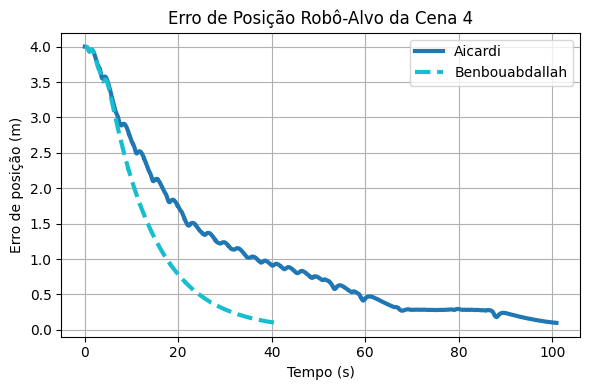
\includegraphics[width=\linewidth]{Figuras/ErroPosição_Cena_4.png}
  \end{minipage}
\end{frame}

\begin{frame}{Erro de Orientação}
  \begin{itemize}
    \item O erro angular $\alpha$ foi avaliado ao longo do tempo.
  \end{itemize}
\end{frame}

\begin{frame}{Erro de Orientação}
\begin{minipage}{0.48\linewidth}
    \centering
    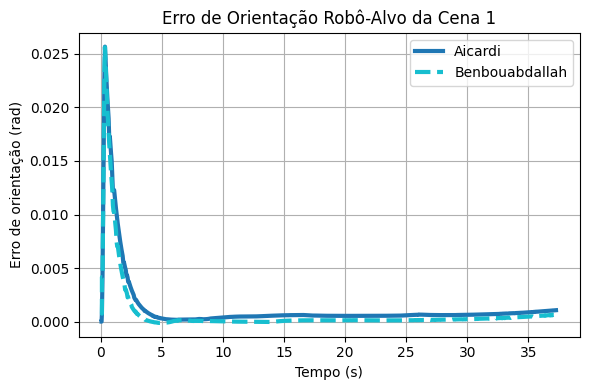
\includegraphics[width=\linewidth]{Figuras/ErroOrientação_Cena_1.png}
  \end{minipage}
  \hfill
  \begin{minipage}{0.48\linewidth}
    \centering
    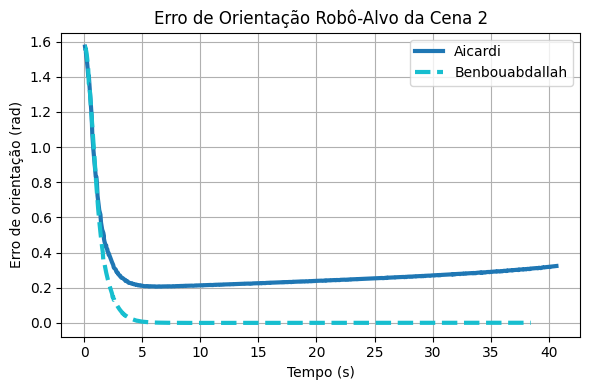
\includegraphics[width=\linewidth]{Figuras/ErroOrientação_Cena_2.png}
  \end{minipage}
\end{frame}

\begin{frame}{Erro de Orientação}
\begin{minipage}{0.48\linewidth}
    \centering
    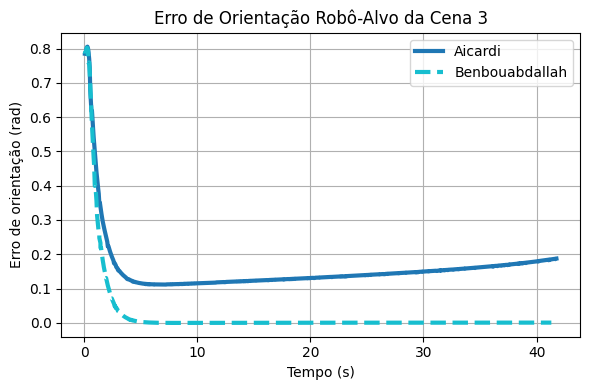
\includegraphics[width=\linewidth]{Figuras/ErroOrientação_Cena_3.png}
  \end{minipage}
  \hfill
  \begin{minipage}{0.48\linewidth}
    \centering
    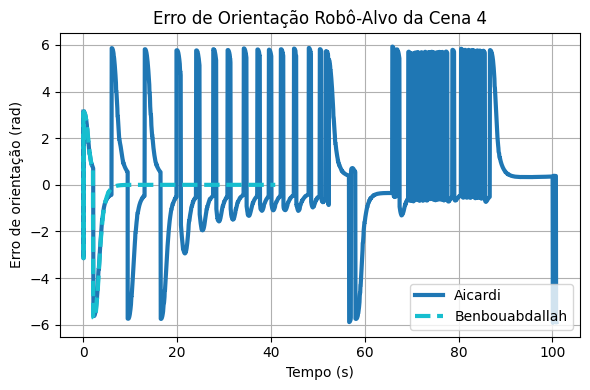
\includegraphics[width=\linewidth]{Figuras/ErroOrientação_Cena_4.png}
  \end{minipage}
\end{frame}

\begin{frame}{Comparação Quantitativa}
  \begin{itemize}
    \item Tempo necessário para alcançar o alvo em cada cena:
  \end{itemize}

  \begin{table}[]
  \centering
  \scriptsize
  \begin{tabular}{|c|c|c|c|c|}
    \hline
    \textbf{Abordagem} & \textbf{Cena 1} & \textbf{Cena 2} & \textbf{Cena 3} & \textbf{Cena 4} \\
    \hline
    Aicardi et al. &  \textbf{37.25} s & 40.65 s & 41.75 s & 100.85 s \\
    Benbouabdallah et al. & 37.35 s & \textbf{38.45 s} & \textbf{41.30 s} & \textbf{40.95 s} \\
    \hline
  \end{tabular}
  \caption{Tempo para o robô atingir o alvo}
  \end{table}
\end{frame}
%======================================================================
% Seção: Conclusão
\section{Conclusão}

\begin{frame}{Conclusões Gerais}
  \begin{itemize}
    \item Ambas as abordagens, Aicardi et al. e Benbouabdallah et al., foram capazes de resolver o problema Go-to-Goal com sucesso.
    \item A estabilidade assintótica foi comprovada teoricamente com base no critério de Lyapunov.
    \item As simulações no CoppeliaSim validaram o comportamento esperado das leis de controle.
  \end{itemize}
\end{frame}

\begin{frame}{Análise Comparativa}
  \begin{itemize}
    \item A abordagem de \textbf{Benbouabdallah et al.} demonstrou desempenho superior na maioria dos testes.
    \item Foi especialmente mais eficaz no caso da Cena 4 (alvo atrás do robô), onde a abordagem de Aicardi teve dificuldade significativa.
    \item A trajetória gerada foi mais direta e o erro de orientação foi menor ao final do movimento.
  \end{itemize}
\end{frame}

\begin{frame}{Considerações Finais}
  \begin{itemize}
    \item O uso da teoria de Lyapunov se mostrou adequado para sistemas não lineares e não-holonômicos.
    \item Resultados indicam que abordagens com estrutura geométrica (como Benbouabdallah) podem ser mais robustas a diferentes configurações iniciais.
  \end{itemize}
\end{frame}
%======================================================================
% Seção: Referências
\section*{Referências}

\begin{frame}{Referências}
  \scriptsize
  \begin{thebibliography}{99}
    \bibitem{aicardi1995}
    Aicardi, M., Casalino, G., Bicchi, A., \& Balestrino, A. (1995).\\
    \textit{Closed loop steering of unicycle-like vehicles via Lyapunov techniques.}\\
    IEEE Robotics \& Automation Magazine, 2(1), 27–35.

    \bibitem{benbouabdallah2013}
    Benbouabdallah, K., \& Zhu, Q. (2013).\\
    \textit{A behavior-based controller for a mobile robot tracking a moving target in multi-obstacles environment.}\\
    In International Conference on Intelligent Human-Machine Systems and Cybernetics, 5(2), 416–422.
  \end{thebibliography}
\end{frame}

% Slide de agradecimento
\begin{frame}[standout]
  \Huge
  \textbf{Obrigado!}

  \vspace{0.5cm}
  \Large
  Perguntas?
\end{frame}

%======================================================================
\end{document}
